\documentclass[journal,twoside,web]{ieeecolor}
% \documentclass[12pt,peerreview,draftversion,onecolumn,print]{ieeecolor}
\usepackage[table,x11names,svgnames,dvipsnames]{xcolor}
\usepackage[export]{adjustbox}
\usepackage{algorithm}
\usepackage[noend]{algpseudocode}
\usepackage{amsmath,amssymb,amsfonts}
\usepackage[USenglish]{babel}
\usepackage{booktabs}
\usepackage{cancel}
\usepackage[tableposition=above]{caption}
% \usepackage{centernot}
% \usepackage{comment}
% \usepackage{enumitem}
\usepackage{epsfig}
\usepackage{epstopdf}
% \usepackage[letterpaper, top=1.0in, bottom=1.0in, left=1.0in, right=1.0in]{geometry}
\RequirePackage[OT1]{fontenc}
% \usepackage{fontspec}
\usepackage{graphics}
\usepackage{graphicx}
\graphicspath{{figures/}}
% \usepackage{ifpdf}
% \usepackage{lastpage}
% \usepackage{leftidx}
\usepackage{lipsum}
% \usepackage{mathrsfs}
\usepackage{mathtools}
% \usepackage{multicol}
% \usepackage{multirow}
\usepackage{nicefrac}
% \usepackage{nicematrix}
% \usepackage{pgfplots}
\usepackage{pifont}
% \usepackage{ragged2e}
% \usepackage{rotating}
% \usepackage{stmaryrd}
% \usepackage[caption=false]{subfig}
\usepackage{tabularx}
\usepackage{tikz}
% \usepackage{tkz-euclide}
% \usepackage{ctable}
% \usetikzlibrary{matrix, arrows}
\usetikzlibrary{shapes.geometric, arrows, angles}
% \usepackage{todonotes}
% \usepackage{wrapfig}

\tikzstyle{startstop} = [rectangle, rounded corners, minimum width=1cm, minimum
height = 0.5cm, text centered, draw=black, fill=red!30]
\tikzstyle{io} = [trapezium, trapezium left angle=70, trapezium right angle=110,
minimum height=1cm, text width=3cm, text centered, draw=black, fill=blue!30]
\tikzstyle{process} = [rectangle, minimum width=2cm, minimum height=0.8cm, text
centered, text width=2cm, draw=black, fill=orange!30]
\tikzstyle{decision} = [diamond, aspect=1.25, minimum width=2cm, minimum height=0.5cm, 
text centered, text width=3cm, draw=black, fill=green!30]
\tikzstyle{arrow} = [thick, ->, >=stealth]




\makeatletter
\newcommand{\rmnum}[1]{\romannumeral #1}
\newcommand{\Rmnum}[1]{\expandafter\@slowromancap\romannumeral #1@}
\makeatother

\newcommand{\bmat}[1]{\begin{bmatrix}#1\end{bmatrix}}
\newcommand{\ubar}[1]{\text{\b{$#1$}}}
\newcommand{\norm}[2]{\|{#1}\|_{{}_{#2}}}
\newcommand{\abs}[1]{\left|{#1}\right|}
\newcommand{\mbf}[1]{\mathbf{#1}}
\newcommand{\mc}[1]{\mathcal{#1}}
\newcommand{\dd}{\operatorname{d}\!}
\newcommand{\muc}[2]{\multicolumn{#1}{c}{#2}}
\newcommand*\Eval[3]{\left.#1\right\rvert_{#2}^{#3}}
\newcommand{\inner}[1]{\left\langle#1\right\rangle}
\newcommand{\pd}[2]{\frac{\partial #1}{\partial #2}}
\newcommand{\pdd}[2]{\frac{\partial^2 #1}{\partial #2^2}}
\newcommand{\el}[2]{\frac{\dd}{\dd t}\pd{\mc{L}}{\dot{#1}} - \pd{\mc{L}}{#1} = #2}
\newcommand{\elk}[2]{\frac{\dd}{\dd t}\pd{\mc{L}}{\dot{#1}_k} - \pd{\mc{L}}{#1_k} = #2_k}
\newcommand{\vectornorm}[1]{\left|\left|#1\right|\right|}
\newcommand{\dom}[1]{\textrm{dom}\;#1}
\newcommand{\bx}{{\bf x}}
\newcommand{\bu}{{\bf u}}
\newcommand{\cmark}{\ding{51}}%
\newcommand{\xmark}{\ding{55}}%

\newcommand{\idapbc}{\textsc{IdaPbc}}

% \theoremstyle{plain}
% \newtheorem{thm}{Theorem}[section]
% \makeatletter
% \@addtoreset{thm}{section}
% \makeatother
% \newtheorem{cor}[thm]{Corollary}
% \newtheorem{lem}[thm]{Lemma}
% \newtheorem{claim}[thm]{Claim}
% \newtheorem{axiom}[thm]{Axiom}
% \newtheorem{conj}[thm]{Conjecture}
% \newtheorem{fact}[thm]{Fact}
% \newtheorem{hypo}[thm]{Hypothesis}
% \newtheorem{assum}[thm]{Assumption}
\newtheorem{prop}{Proposition}
% \newtheorem{crit}[thm]{Criterion}
% \theoremstyle{definition}
% \newtheorem{defn}[thm]{Definition}
% \newtheorem{exmp}[thm]{Example}
\newtheorem{rem}{Remark}
% \newtheorem{prin}[thm]{Principle}

\DeclareMathOperator{\Tr}{tr}
\newcommand\xdownarrow[1][2ex]{%
   \mathrel{\rotatebox{90}{$\xleftarrow{\rule{#1}{0pt}}$}}
}
\DeclareMathOperator{\End}{End}
\DeclareMathOperator{\Hom}{Hom}
\DeclareMathOperator{\id}{id}
\DeclareMathOperator{\vers}{vers}
\DeclareMathOperator{\trans}{Trans}
\DeclareMathOperator{\rot}{Rot}
\DeclareMathOperator{\rank}{rank}
\DeclareMathOperator{\sinc}{sinc}

%% The section below needs to be put at the end of this file to make citation links work with ieeeconf.cls
\makeatletter
\let\NAT@parse\undefined
\makeatother
\usepackage{hyperref}
\hypersetup{
    unicode=false,          % non-Latin characters in Acrobat’s bookmarks
    pdftoolbar=true,        % show Acrobat’s toolbar?
    pdfmenubar=true,        % show Acrobat’s menu?
    pdffitwindow=false,     % window fit to page when opened
    pdfstartview={FitH},    % fits the width of the page to the window
    pdftitle={Robust Interconnection and Damping Assignment Passivity-Based Control via Neural Bayesian Inference},    % title
    pdfauthor={Wankun Sirichotiyakul, Nardos Ayele Ashenafi, Aykut C. Satici},     % author
    % pdfsubject={Subject},   % subject of the document
    % pdfcreator={Creator},   % creator of the document
    % pdfproducer={Producer}, % producer of the document
    % pdfkeywords={keyword1, key2, key3}, % list of keywords
    pdfnewwindow=true,      % links in new PDF window
    colorlinks=true,       % false: boxed links; true: colored links
    linkcolor=magenta,          % color of internal links (change box color with linkbordercolor)
    linkbordercolor=orange,
    citecolor=blue,        % color of links to bibliography
    citebordercolor=green,
    filecolor=magenta,      % color of file links
    urlcolor=cyan,           % color of external links
    urlbordercolor=blue,
}

\usepackage{generic}

% Not sure if needed
\def\BibTeX{{\rm B\kern-.05em{\sc i\kern-.025em b}\kern-.08em
    T\kern-.1667em\lower.7ex\hbox{E}\kern-.125emX}}

\markboth{\journalname, VOL. XX, NO. XX, July 2022}
{Simple Geometry Question}

\begin{document}

\title{Simple Geometry Problem} 
\author{
%     Wankun Sirichotiyakul, \IEEEmembership{Student Member, IEEE};
%     Nardos Ayele Ashenafi, \IEEEmembership{Student Member, IEEE};\\%
    Aykut C. Satici, \IEEEmembership{Member, IEEE}
%     \thanks{Submitted for review on 6 April 2022.}
%     \thanks{W. Sirichotiyakul and N. A. Ashenafi are with the Electrical and Computer Engineering Department, Boise State University, Boise, ID 83706 USA
%     (e-mail: \{wankunsirichotiyakul,nardosashenafi\}@boisestate.edu).}
    \thanks{A. C. Satici is with the Mechanical and Biomedical Engineering Department, Boise State University, Boise, ID 83706 USA
    (e-mail: aykutsatici@boisestate.edu).}
}
\maketitle
% \IEEEpeerreviewmaketitle

  
\begin{abstract} % Abstract of not more than 200 words.

This simple geometry problem is my excuse to teach myself some Ti\textit{k}Z.

\end{abstract}

\begin{IEEEkeywords}
  Geometry, Ti\textit{k}Z
\end{IEEEkeywords}

\section{Introduction}
\label{sec:intro}

I saw this problem in P. Talwalkar's YouTube channel~\cite{mindyourdecisions}.

\section{Problem Statement}
\label{sec:statement}

% \begin{center}
% \begin{tikzpicture}[scale=1.75, every node/.style={scale=0.75}]
%   \clip (-1.1,-0.5) rectangle (4.8,4.2);
%   \draw[thin] (0,0) rectangle (4,3);
%   \draw (0,0) -- (4,3);
%   \draw (1.0, 2.0) circle [radius=1cm];
%   \draw (3.0, 1.0) circle [radius=1cm];
%   \draw (1.0, 2.0) -- (3.0, 1.0);
%   \filldraw (1.0, 2.0) circle [radius=0.2mm];
%   \filldraw (3.0, 1.0) circle [radius=0.2mm];
%   \draw (1.0,2.0) node[above left] {$X$};
%   \draw (3.0,1.0) node[below] {$Y$};
%   \draw (2.0,0.0) node[below] {$w$};
%   \draw (4.0,1.5) node[right] {$h$};
% \end{tikzpicture}
% \end{center}

The original problem is stated as in the caption of Figure~\ref{fig:problem}.
However, we will extend the statement slightly to make it a tiny bit more
interesting.  Let $r$ be the radius of the circles and pose the following
questions:

\begin{figure}[h]
  \centering
  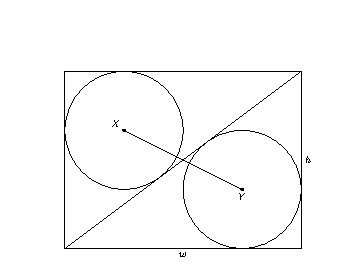
\includegraphics[trim={0 0 0 1.2cm},clip,width=0.5\textwidth]{./figures/basic1.pdf}
  \vspace{-8mm}
  \caption{Given the width $w$ and height $h$ of the rectangle, find the length
  of the line segment $XY$ between the centres of the inscribed circles, which
  have the two adjacent sides of the rectangle and its diagonal as tangents.}
  \label{fig:problem}
\end{figure}

\begin{enumerate}
  \setlength\itemsep{0em}
  \item Find the map $f: \mathbb{R}_+^2 \rightarrow \mathbb{R}_+^2$ that takes
          the side lengths of the rectangle $(w,h)$ to $(r, \abs{XY})$, the
          radius of one of the circles and the length of the line segment $XY$.
  \item Find the inverse $f^{-1}$ of $f$, that takes $(r, \abs{XY})$ to $(w,h)$.
\end{enumerate}


\section{Problem Solution}
\label{sec:solution}

We will make use of Figure~\ref{fig:solution} in the following derivation.
The diagonal length $d \triangleq \abs{AC}$ of the rectangle is given by 
%
\begin{equation}
  d^2 = w^2 + h^2.
  \label{eq:diagsq}
\end{equation}
%
\begin{figure}[h]
  \centering
  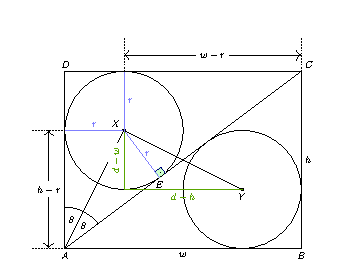
\includegraphics[trim={0 0 0 0.55cm},clip,width=0.5\textwidth]{./figures/basic2.pdf}
  \vspace{-8mm}
  \caption{Auxiliary drawing, identifying key lengths and angles.}
  \label{fig:solution}
\end{figure}
%
The diagonal length $d$ may also be related to $(w,h)$ and $r$ by noting that
$\abs{AE} = h-r$ and $\abs{EC} = w-r$ due to the tangency to the circles. On the
other hand, $d = \abs{AC} = \abs{AE} + \abs{EC}$ so that 
%
\begin{equation}
  d + 2r = w + h.
  \label{eq:diaglin}
\end{equation}

\subsection{Computing $\abs{XY}$, given $w$ and $h$}
\label{ssec:compute_xy}

In order to compute $\abs{XY}$, form the right triangle whose horizontal and
vertical sides are drawn in green in Figure~\ref{fig:solution}. The length of
the vertical side of this triangle is $h-2r$ but by equation~\eqref{eq:diaglin}
this is equal to $d-w$. Similarly, the length of the horizontal side of this
triangle is $w-2r$ but, by the same token, this is equal to $d-h$. Hence, we
have
%
\begin{equation}
  \abs{XY}^2 = (d-w)^2 + (d-h)^2 = 3d^2 - 2d(w+h),
  \label{eq:xylen}
\end{equation}
%
where the second equality may be derived by substituting from
equation~\eqref{eq:diagsq}.

\subsection{Computing $r$, given $w$ and $h$}
\label{ssec:compute_r}

The right triangle $\triangle CAD$ provides the equality \[ \tan{2\theta} =
\frac{2\tan{\theta}}{1-\tan^2{\theta}} = \frac{w}{h}, \] which implies the
quadratic equation \[ \tan^2{\theta} + 2\nicefrac{h}{w}\tan{\theta} - 1 = 0. \]
Solving for $\tan{\theta}$ such that $0 < \theta < \nicefrac{\pi}{2}$, we obtain
\[ \frac{r}{h-r} = \tan{\theta} = \nicefrac{1}{w}(d-h), \] where the first 
equality follows from the right triangle $\triangle EAX$. We can solve this
equation for the radius, $r$, which provides the solution
%
\begin{equation}
  r = \frac{h(d-h)}{w+d-h}.
  \label{eq:radius}
\end{equation}

\subsection{Computing $f$ and its inverse $f^{-1}$}

The development of Sections~\ref{ssec:compute_r} and~\ref{ssec:compute_xy}
readily yields $f: \mathbb{R}_+^2 \rightarrow \mathbb{R}_+^2$.
%
\begin{align}
  \begin{split}
    d &= \sqrt{w^2 + h^2}, \\
    f(w,h) &= \left( \frac{h(d-h)}{w+d-h}, \sqrt{(d-w)^2 + (d-h)^2} \right).
  \end{split}
  \label{eq:f}
\end{align}
%
In order to look for its inverse, let us recall equation~\eqref{eq:xylen} and
substitute from~\eqref{eq:diaglin} for $w+h$, yielding the relationship 
\begin{equation} 
 d^2 - 4rd - \abs{XY}^2 = 0, 
 \label{eq:dquad}
\end{equation}
%
which implies 
%
\begin{equation}
  d = 2r + \sqrt{\abs{XY}^2 + 4r^2}, 
  \label{eq:inversed}
\end{equation}
%
since $d > 0$. Let us solve for $h$ from equation~\eqref{eq:diaglin} and
substitute into equation~\eqref{eq:diagsq}, which yields \[ w^2 - (2r+d)w +
2r(r+d) = 0. \] Now, if we notice that equations~\eqref{eq:diagsq}
and~\eqref{eq:diaglin} are both symmetric in $w$ and $h$, then we can deduce
that the two solutions of this quadratic equation correspond to $w$ and $h$.
Assuming, without loss of generality, $w > h$, and substituting
from~\eqref{eq:dquad} and~\eqref{eq:inversed}, we obtain 
%
\begin{align*}
  w(r,\abs{XY}) &= \nicefrac{1}{2}\left(2r+d + \sqrt{d^2 - 4rd - 4r^2} \right) \\ 
    &= 2r + \nicefrac{1}{2} \left( \sqrt{\abs{XY}^2 + 4r^2} + \sqrt{\abs{XY}^2 -
4r^2} \right),
\end{align*}
%
and 
%
\begin{align*}
  h(r,\abs{XY}) &= \nicefrac{1}{2}\left(2r+d - \sqrt{d^2 - 4rd - 4r^2} \right) \\ 
    &= 2r + \nicefrac{1}{2} \left( \sqrt{\abs{XY}^2 + 4r^2} - \sqrt{\abs{XY}^2 -
4r^2} \right),
\end{align*}
%
which yields the inverse function $f^{-1}(r,\abs{XY}) = (w,h)$.

\section{Conclusion}
\label{sec:conclusion}

This has been a nice excuse to practice some Ti\textit{k}Z.


\bibliographystyle{ieeetr}        
\bibliography{bib/basicgeo.bib}  

% \appendix

\newcommand*{\bbU}{\mathbb{U}}

\subsection{Computing the angle $\theta$ and $r$ from it}

The right triangle $\triangle CAD$ provides the equality \[ \tan{2\theta} =
\frac{2\tan{\theta}}{1-\tan^2{\theta}} = \frac{w}{h}, \] which implies the
quadratic equation \[ \tan^2{\theta} + 2\nicefrac{h}{w}\tan{\theta} - 1 = 0. \]
Solving for $\tan{\theta}$ such that $0 < \theta < \nicefrac{\pi}{2}$, we obtain
\[ \frac{r}{h-r} = \tan{\theta} = \nicefrac{1}{w}(d-h), \] where the first 
equality follows from the right triangle $\triangle EAX$. We can solve this
equation for the radius, $r$, which provides the solution
%
\begin{equation}
  r = \frac{h(d-h)}{w+d-h}.
  \label{eq:radiusalt}
\end{equation}
%
Simple computation shows that 
\[ \frac{h(d-h)}{w+d-h} = \nicefrac{1}{2}(w+h-d). \]


\end{document}
